\subsection{Experiment Settings}

\begin{table}[t]
    \centering
        \caption{Characteristics of datasets and privacy parameters}
    \scalebox{0.85}{
        \begin{tabular}{|l|c|c|c||c|}
        \hline 
        \textbf{Name} & \textbf{Content}  & \textbf{Nodes}    & \textbf{Edges}  & \textbf{$\epsilon$} \\
        \hline 
        \hline  
        \textrm{PPI} & \footnotesize{Protein-protein Interaction}  &12K       &397K        &$10^{-2}$\\
        \textrm{BK}  & \footnotesize{Location-based OSN}    &58K       &214K        &$10^{-3}$ \\
        \textrm{DBLP}& \footnotesize{Co-authorship Network} & 824K      &5M         & $10^{-4}$\\
        \hline
        \end{tabular}
     }
        \label{tab:dataset}
    \vspace{-10pt}
\end{table}


\textbf{Datasets}~~We test three obfuscation methods on three uncertain graphs: PPI, BrightKite (BK) and DBLP as described in Table \ref{tab:dataset}. These datasets have been widely used in the study of uncertain graphs~\cite{Zhao_Detecting_2014,Potamias_K_2010,Jin_Distance_2011}. 

% \begin{itemize}
% 	\item{PPI is a dataset of protein-protein interactions, provided by Disease Module Identification DREAM Challenge. The probability of any edge corresponds to the confidence that the interaction actually exists, which is obtained through biological experiments.}
% 	\item{BrightKite (BK) is a location-based social network. In this dataset, each node represent a user. The probability of any edge corresponds to the chance that two users visit each other.}
% 	\item{DBLP is a dataset of scientific publications and authors. Each node represent an author. Two authors are connected by an edge if they have co-authored in a project. The uncertainty on the edge denotes the likelihood that the two authors will collaborate in a new project.}
% \end{itemize}
\begin{figure}[!t]
	\begin{flushleft}
	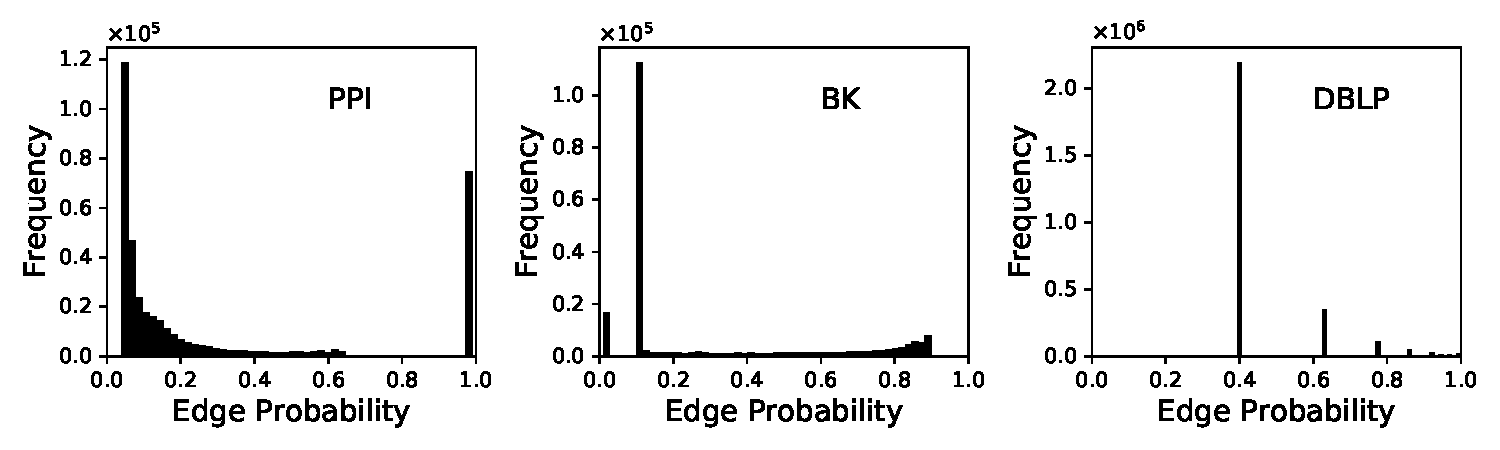
\includegraphics[height=2.6cm]{expResult/probDistribution.pdf}
	\end{flushleft}
	\vspace{-10pt}
	\caption{Edge probability distributions.}
	\vspace{-10pt}
\end{figure}
\begin{figure}[!t]
	\begin{flushleft}
	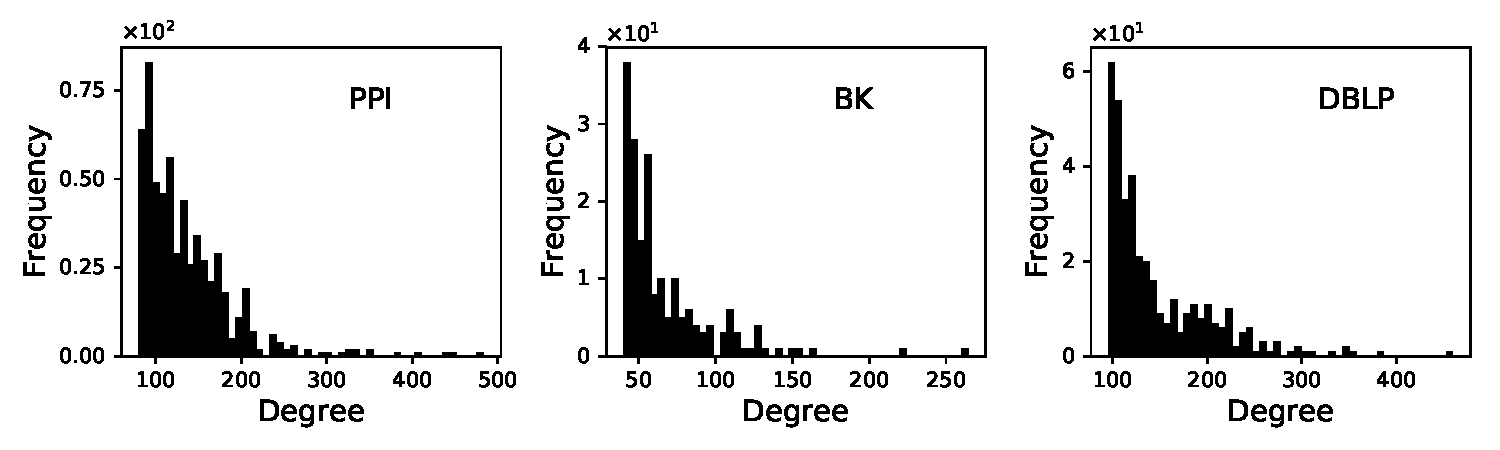
\includegraphics[height=2.6cm]{expResult/degDistribution.pdf}
	\end{flushleft}
	\vspace{-10pt}
	\caption{Degree distributions.}
	\label{fig:degreeDist}
	\vspace{-10pt}
\end{figure}
Note that edge probability values of BrightKite and DBLP are obtained by prediction models built on historical logs which contain sensitive and confidential information. 
These graphs not only capture different real-world scenarios but also different data characteristics {\eg}, size, density, edge probability. 
The graphs size vary from 12K of PPI,  58K of BK, to 824K of DBLP with different densities; 
DBLP is the largest but also the sparest dataset.  
The probability values of PPI and BrightKite are generally very small. 
The PPI dataset has a more uniform probability distribution. While, DBLP dataset only has a few probability values.

We report their degree distributions of “unique” nodes whose obfuscation level is smaller than 300 in Figure~\ref{fig:degreeDist}. Observe that, all the three graphs have a heavy-tailed degree distribution. Namely, they are difficult to be obfuscated.

\textbf{Parameter Setting}~~We consider various obfuscation levels, $k \in \{100,150,200,250,300\}$ and possible tolerance values $\epsilon$ to explore the performance difference. 

\textbf{Statistics}~~For every uncertain graph (obfuscated outputs and original ones), we sampled $N$ possible worlds to compute its statistics of interest. Note that it has been shown that 1000 possible worlds usually suffices to achieve accuracy converge.  Then, we compute the discrepancy of obfuscated outputs against the original one. The smaller discrepancy, the better uncertain graph data utility preserving.


